\subsection{Battery Discharge}

The 12 volt 12 amp hour lithium ion batteries were tested to determine how long our system would last running only on battery power.  The specifications from Appendix \ref{fig:battspec} show the discharge rates, voltage cutoff, and how capacity varies over charge cycles.

\indent First a Sylvania 3157 automotive light bulb was tested. The light bulb is rated for 26.88 watts.  The voltage was recorded as the light bulb discharged the battery. The battery started off at 13.21 volts and discharged for 10:19:39 where it cut out at 9 volts. The light bulb draws more current than the projected package and it was decided to switch to a higher resistance load.
 
\indent A pair of 100 $\Omega$ resistors were connected in parallel to achieve a measured resistance of 49.65  $\Omega$. At 12 volts the resistor will dissipate 2.88 watts of power, identical to the predicted power consumption of the package.  The battery started at 13.2 volts and discharged for 20:22:12 where it cut out at 9 volts. 

\indent Figure \ref{fig:discharge} shows the comparison of the two loads. The shapes of the curves are identical. Decreasing the load resulted in 

\indent Current monitoring will be required to produce more accurate power curves. 

\begin{figure}
\centering
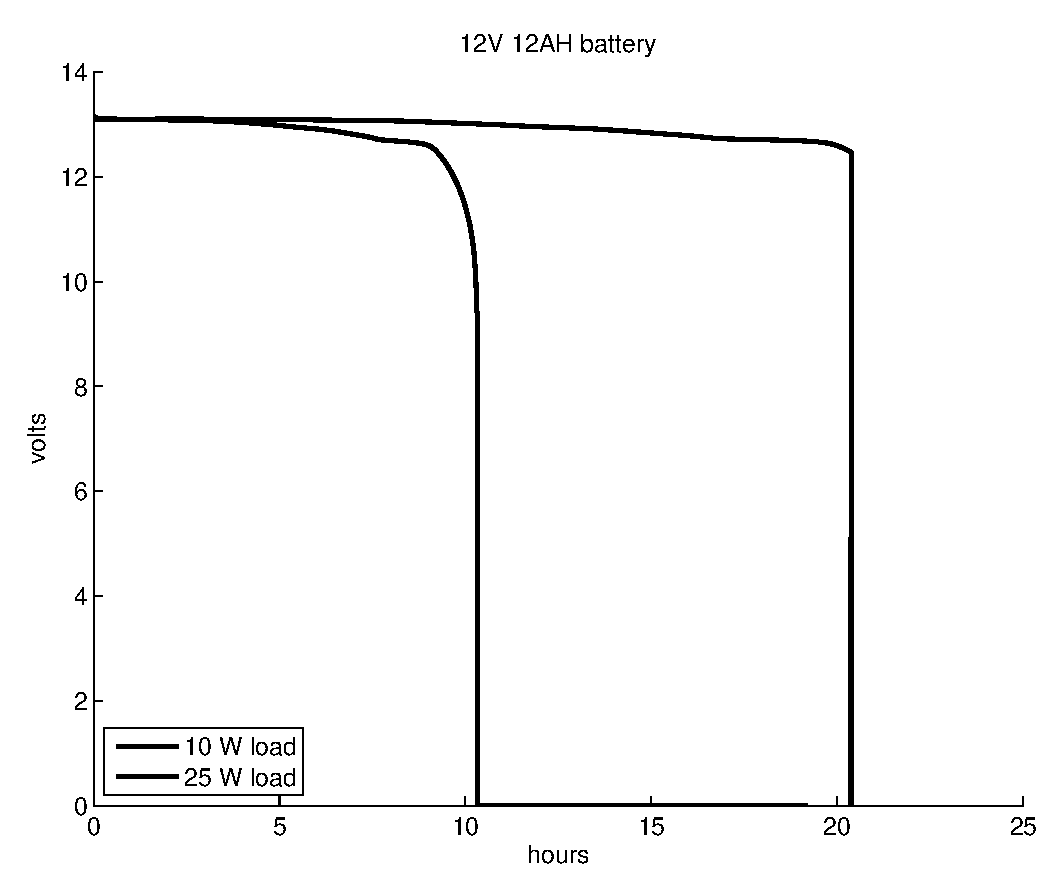
\includegraphics[width=\textwidth]{WESLEY_dischargecurves.eps}
 \caption{\textit{Discharge of batteries with 2 loads}}
\label{fig:discharge}
\end{figure}
